\documentclass[11pt,letterpaper]{article}

%\usepackage{subfigure}
\usepackage{graphicx}
\usepackage{amsmath}
\usepackage{amssymb}
\usepackage{enumitem}
\usepackage{setspace}
\usepackage{paralist}
%\usepackage{amsmath}
\usepackage{bm}
%\usepackage{subfigure}
\usepackage{cite}
\usepackage{multirow}
\usepackage{todonotes}
\usepackage{umoline}
\usepackage{xspace}
\usepackage{soul}
\usepackage{graphicx}
\usepackage{url}

\usepackage{paralist}

%\usepackage{gensymb}
%\usepackage[euler]{textgreek}
%\usepackage{array}
%\usepackage{tabu}
%\usepackage{tabularx}
\usepackage{subcaption}
%\usepackage{amsmath}
%\usepackage{cleveref}


\setlength{\textwidth}{6.5in}     
\setlength{\oddsidemargin}{0in}  
\setlength{\evensidemargin}{0in}
\setlength{\textheight}{8.5in} 
\setlength{\topmargin}{0in}   
\setlength{\headheight}{14pt} 
\setlength{\headsep}{10pt}   
%\setlength{\footskip}{0in}

%------------------------------------------------
\newcommand{\homework}[2]{
\setcounter{section}{#1}
\section*{ICS635 Homework {\thesection}: {#2} }
{\markboth{#2}{#2}}
}
%------------------------------------------------


\begin{document}

% Enter the Homework number and title as arguments to
% homework
%\homework{3}{by Lambert Leong}
\title{ICS635 Homework 3}
\author{Lambert Leong}
\maketitle
\section{Introduction}
I chose to participate in the Santander Customer Transaction competition.  A
quick survey of the raw training data revealed that there are 200 features which
contain positive or negative float values.  My initial thought was to perform a
principal components analysis (PCA) to try and reduce the dimensionality of the
data.  Several visualization kernerls showed that the distribution for each
class with respect to each field, i.e. `var\_0', `var\_1',etc..., is not very
different.  In fact, there is a significant overlap of the two classes for
almost all features and determining a decision boundary appears to be non-trivial.
This lead me to believe that mapping the data into a new space with PCA would
not be useful for the purposes of reducing data dimensionality.

% looked at visualization kernels
% Noticed that each variable was not really seperable
% Wondered if PCA could reduce dimensionality
%  - turns out it didnt really work...

% Gradient boosting to start
% enought data to split training and val
I first looked at an ensembling methods and used gradient boosting to classify
the data as is, with all 200 features.  I then used the same gradient boosting
classifier on training data which had the dimensionality reduced via PCA.
Comparing the results of the original data, with 200 features, to the PCA
transformed data, with less than 200 features, indicated that I should not
proceeds with PCA and models generated with all 200 features were able to
generalize to the validation set better.

\iffalse
% Noticed the data description said that amount is irrelavant
% thought maybe we could view the data as sequence data
%  - extract patterns in transaction histories
% assumes its a time series and assumed there was a particular order
% 1D CNN and LSTM
The instructions on the competetion website stated,``...identify which customers
will make a specific transaction in the future, irrespective of the amount of
money transacted.'' From these instruction I hypothesized that each feature
could represent a transaciton from an individual's transaction history and I
looked into treating the data as sequence data.  I explored two neural network
architectures which include long short term memory (LSTM) recurrent neural
network and a 1D convolutional neural network (CNN).  The motivation behind
implementing these neural networks was to try to explore patterns in the
sequence of transacitons that may correlate to a particular class.
\fi

% feature engineering
% count pos and neg
% mean, std, skew, kurtosis
% longest pos and neg seq
The instruction also noted that the transaction amount is not really relavent.
Each of the 200 feature fields contained either a positve or negative number
which could indicate money coming in and money going out, respectively.  Under
this assumption, I sought to capture the amount of times money came in and the
number of times money went out for a particular individual to see if it had any
correlation to a particular class.  In other words, I captures the total amount
of postive values and the total amount of negative values for each individual in
the dataset.  

Although it is stated that the ammount of the transaction is not relavent I
added features that indirectly correlate to the amount and these features
include mean, standard deviation, skew, and kurtosis.  I applied the previously
mention models, gradiant boosting, LSTM, and 1D CNN, to the new dataset with new
features to see if it would lead to better classification. 

\section{Methods}
The first thing that was done was to split the training data into a training and
validation set.  The Scikit-learn train\_test\_split function was used to split
the training data.  A random\_state of 18 was used and the test size was 0.2
which resulted in 80\% of the original training data to be used for training and
the remaining 20\% to be used for validation.  

\subsection{PCA}
%PCA
% - centered data
PCA was performed using Scikit-lean's decomposition module.  PCA was performed
on centered and non-centered data which yeilded similar results.  I sought to
reduce the number of features by keeping those which explain 95\% of the
variance.  It turns out that 118 features explain about 95\% of the total
variance which is more features than what was initially expected.  The top 118
features were kept and used to train a gradient boosting model.
 
\subsection{Gradient Boosting}
% XGBoost
% - on pca and non pca data sets
The sklearn xgboost module was used to create the gradient boosting model. The
model was trained and evaluated on the original training data, with all 200
features, as well as with the PCA reduced data with 118 features.  Area under
reciever operation characteristic (AUROC) was used to evaluate how well the
model was at generalizing to the validation test set.  The non-reduced data, the
original data yeilded higher AUROC values, at around 0.885, when compared to the
models trained on PCA transformed data.  Different numbers of features were
experiemented with for PCA but the full dataset still yield the best results.

\subsection{Feature Engineering}
% XGBoost with new feat
% - parameters tuning
Functions were written to itterate through each row or record and count the
number of positive values and the number of negative values.  These two numbers
were appended to the end of the dataset as two extra features.  Another function
was written to capture the longest sequence, within each row, of positive
numbers and negative numbers.  These features were engineered under the
hypothesis that this could be sequence data and under the assumption that the
order of the features have not been randomized. 

\subsection{Parameter Tuning}
Model parameters, which include n\_estimators, max\_depth, and the learning rate
were choosen with the help of the GridSearchCV.  GridSearchCV exhaustively
searches through a range of choosen values for each of the model parameters and
helps you choose the best parameter values.  Parameters and their final values
are as follows: n\_estimators = 1500, max\_depth = 3, and the learning rate =
0.3. The tree\_method was gpu\_hist and predictor was gpu\_predictor; these
parameters were not tunned and choosen so that GPU acceleration could be
enabled.   

\iffalse
\subsection{Neural Networks}
% 1D CNN

% LSTM
\fi

\section{Results}

\begin{figure}[h!]
    \centering
    \begin{subfigure}[]{.4\textwidth}
        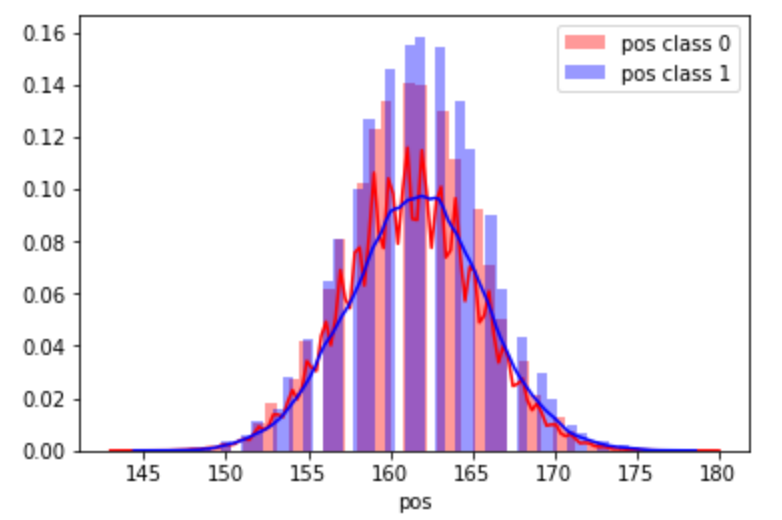
\includegraphics[width=\textwidth]{pos_dist.png}
        \caption{Distribution of postitive numbers by class}
        \label{fig:pos_dist}
    \end{subfigure}
    \begin{subfigure}[]{.4\textwidth}
        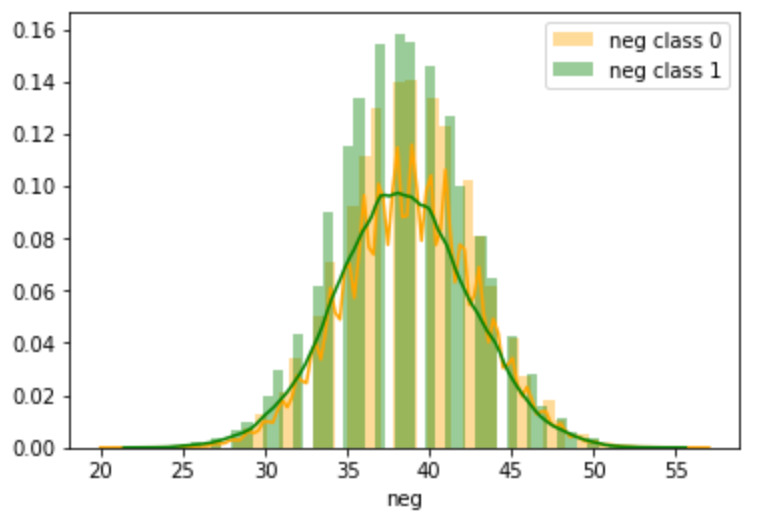
\includegraphics[width=\textwidth]{neg_dist.png}
        \caption{Distribution of negative numbers by class}
        \label{fig:neg_dist}
    \end{subfigure}
    \caption{Frequency distributions for postive and negative values colored by
class}
    \label{fig:count_dist}
\end{figure}

\begin{figure}[h!]
    \centering
    \begin{subfigure}[]{.4\textwidth}
        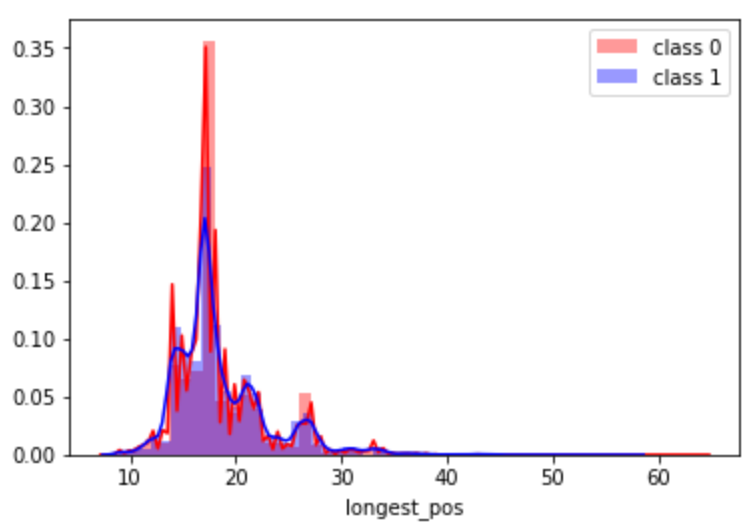
\includegraphics[width=\textwidth]{long_pos_dist.png}
        \caption{Distribution of postitive numbers by class}
        \label{fig:pos_dist}
    \end{subfigure}
    \begin{subfigure}[]{.4\textwidth}
        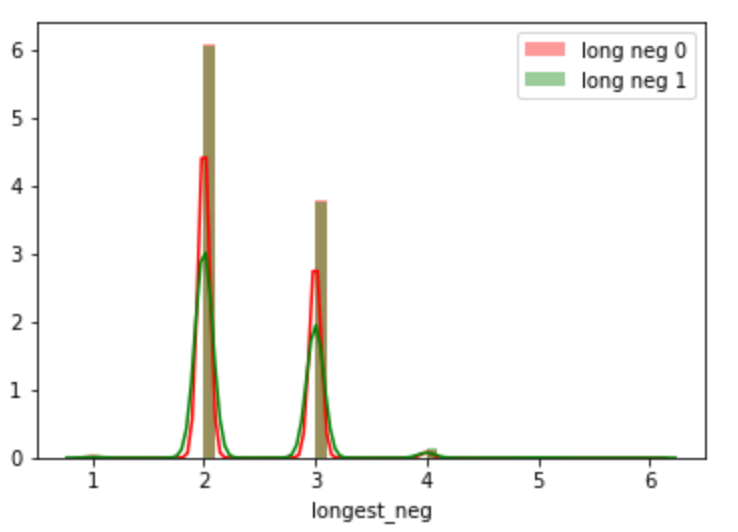
\includegraphics[width=\textwidth]{long_neg_dist.png}
        \caption{Distribution of negative numbers by class}
        \label{fig:neg_dist}
    \end{subfigure}
    \caption{Frequency distributions for longest postive sequence and longest
negative sequence values colored by class}
    \label{fig:count_dist}
\end{figure}

\begin{table}[h!]
\begin{tabular}{|c|c|}
\hline
Model & Best Public Score \\ \hline
1D CNN & 0.833 \\ \hline
LSTM & 0.829 \\ \hline
PCA XGBoost & 0.882 \\ \hline
XGBoost & 0.899 \\ \hline
\end{tabular}
\end{table}

\section{Conclusion}
\end{document}
